% Chapter 2
\chapter{Background}\label{ch:background} % For referencing the chapter elsewhere, use \autoref{ch:examples} 
\minitoc% Creating an actual minitoc\
\bigskip

In this chapter, we describe the main concepts and principles behind observability in distributed systems and anomaly detection. We relate the modern distributed systems, the observability data, and the anomaly detection, and provide overview of the main solutions presented in the thesis within a proposed reference architecture. 

\section{Distributed Systems Observability}
A distributed system is a system with multiple components located on different machines that communicate and coordinate actions over the network by passing messages to one another~\cite{tanenbaum2007distributed}
An example of a distributed system is a system based on Service-Oriented Architectures (SOA). At the time of writing this thesis, SOA were introduced almost 25 years ago~\cite{abrams2008service}. Since then, the field has been actively researched, leading to a huge paradigm shift. Recently, a variant of SOA, called microservice architectures emerged as a standard architecture for software systems. However, precisely defining the conceptual difference between microservice architectures and SOA is difficult, as microservices are often seen as a reinvention of the almost outdated SOA principles. Today, more than two decades after the introduction of SOA, systems based on microservices are state-of-the-art, and major companies such as Google, Twitter, and Amazon, had already seen the benefits of breaking their monoliths into distributed components~\cite{observability2020practical}. Furthermore, cloud providers such as Amazon Web Services (AWS) and Microsoft Azure enabled companies to move their infrastructure into the cloud, where ideas like microservices are easy to implement. This facilitated the general paradigm shift in software. 

This conceptual change in software architecture means that the services increasingly rely on intra-system communication, making these highly distributed systems even more complex. The increased complexity of having highly distributed architecture leads to difficulty in system operation and maintenance, which directly affects their reliability, availability, resilience, and security.
Availability is a characteristic of a system, which aims to ensure an agreed level of operational performance, usually uptime, for a higher than normal period. Reliability is the probability of continuous correct operation. 

Building reliable and resilient systems require context-aware monitoring of the distributed infrastructure, which is often called observability. Distributed systems are inherently designed not to be available all the time at 100\%~\cite{gunawi2014bugs}. Therefore, collecting every possible snapshot of the system, which can be then used to develop intelligent analytics and prediction tools to support troubleshooting and operations such as anomaly detection, root-cause analysis, and probably self-healing triggers into the system. 

Observable systems require the collection of factual data and extracting insightful information. The distributed system data comes in the form of logs, traces, and metrics are often known as the three pillars of observability~\cite{nedelkoski2020data,observability2020practical}.
Logs enable developers to record what actions were executed at runtime by software. Services and other systems generate logs that are composed of timestamped records with a structure and free-form text.
Distributed traces record the workflows of services executed in response to requests, e.g., HTTP or RPC requests. The records contain information about the execution graph and performance at a microservice level. Metrics are numeric values measured over a while. They describe the utilization and status of the infrastructure, typically regarding CPU, memory, disk, network throughput, and service call latency. 

We note that these major observability components can be instrumented and available for any distributed software system, as they comply with modern software engineering practices~\cite{sridharan2018distributed}.

\subsection{Logs} 
Recent software engineering research has demonstrated the importance of logs in understanding and improving software systems. For example, system operators leverage the rich information in logs to generate workload information for capacity planning in large-scale systems~\cite{hassan2008industrial,nagappan2009efficiently}, monitor the overall system health~\cite{jiang2013automated}, perform anomaly detection~\cite{meng2019loganomaly,nedelkoski2019anomaly,nedelkoski2020loganomaly,nedelkoski2020selfsupervised,du2017deeplog,zhang2019robust,du2016spell,zhu2019tools}, analyze the root cause of a problem~\cite{Yuan2019AnAT,zhou2019latent,chen2019empirical}, reproduce failures~\cite{zhang2017pensieve}, improve performance, reduce energy consumption, deal with security issues~\cite{zhao2016non}, reconstruct workflows~\cite{bao2019miningworkflows}, and discover bugs~\cite{mohan2018finding}, among other applications. 

Logs are not only used as a benefit of developers and operators for successfully managing the system, but they are often needed to comply with legal regulations. For example, the Sarbanes-Oxley Act of 2002 specifies that the execution of telecommunication and financial applications must be logged to help protect the general public from errors and fraudulent practices.

In modern complex distributed systems, logs provide vital insight by capturing the state of the system for each service/component. Logs are generally instrumented as per their usability by developers. Depending on the storage rules, they are processed, aggregated, and ultimately stored in a centralized data store from where they can be analyzed. Regarding the origin from which logs appear, there can be from application logic code, middleware, network communications (e.g., from switches), database communication, message brokers, caches, interaction with load balancers, and communication with security and authentication modules. 

Independent of their origin type, logs often contain free-form text with a timestamp, alongside other system-dependent fields. We show few typical log messages from a cloud computing infrastructure software (OpenStack~\cite{openstack}) in Figure~\ref{fig:log_lines}. The first field is the host name (wally\[number\]), it is followed by a timestamp when the log was generated, log level (e.g., INFO, WARNING, ERROR, etc.), the payload or the actual print statement written by developers, and the name of the service from which was generated. Regarding the service, we observe log messages from three different services within the system, namely, \textit{compute claims}, \textit{compute.manager}, and \textit{virt.libvirt.driver}, all related to the execution of a user request of creating a virtual machine in the cloud. The free-form message or the log payload contains most of the meaningful information, while the timestamp gives the context of surrounding log messages, useful when troubleshooting. 

Log data analysis is often based on understanding the free-form text. Experienced developers and operators with understanding of the system can detect if there is problem that can be observed in the logs. However, as explained in Chapter~\ref{ch:introduction}, due to the massive amounts of log data, manual inspection is often infeasible. For automated analysis there are some inherent properties of these systems that are reflected in the log data that increase the difficulty of the aforementioned tasks 

\begin{figure}[htbp]
\centerline{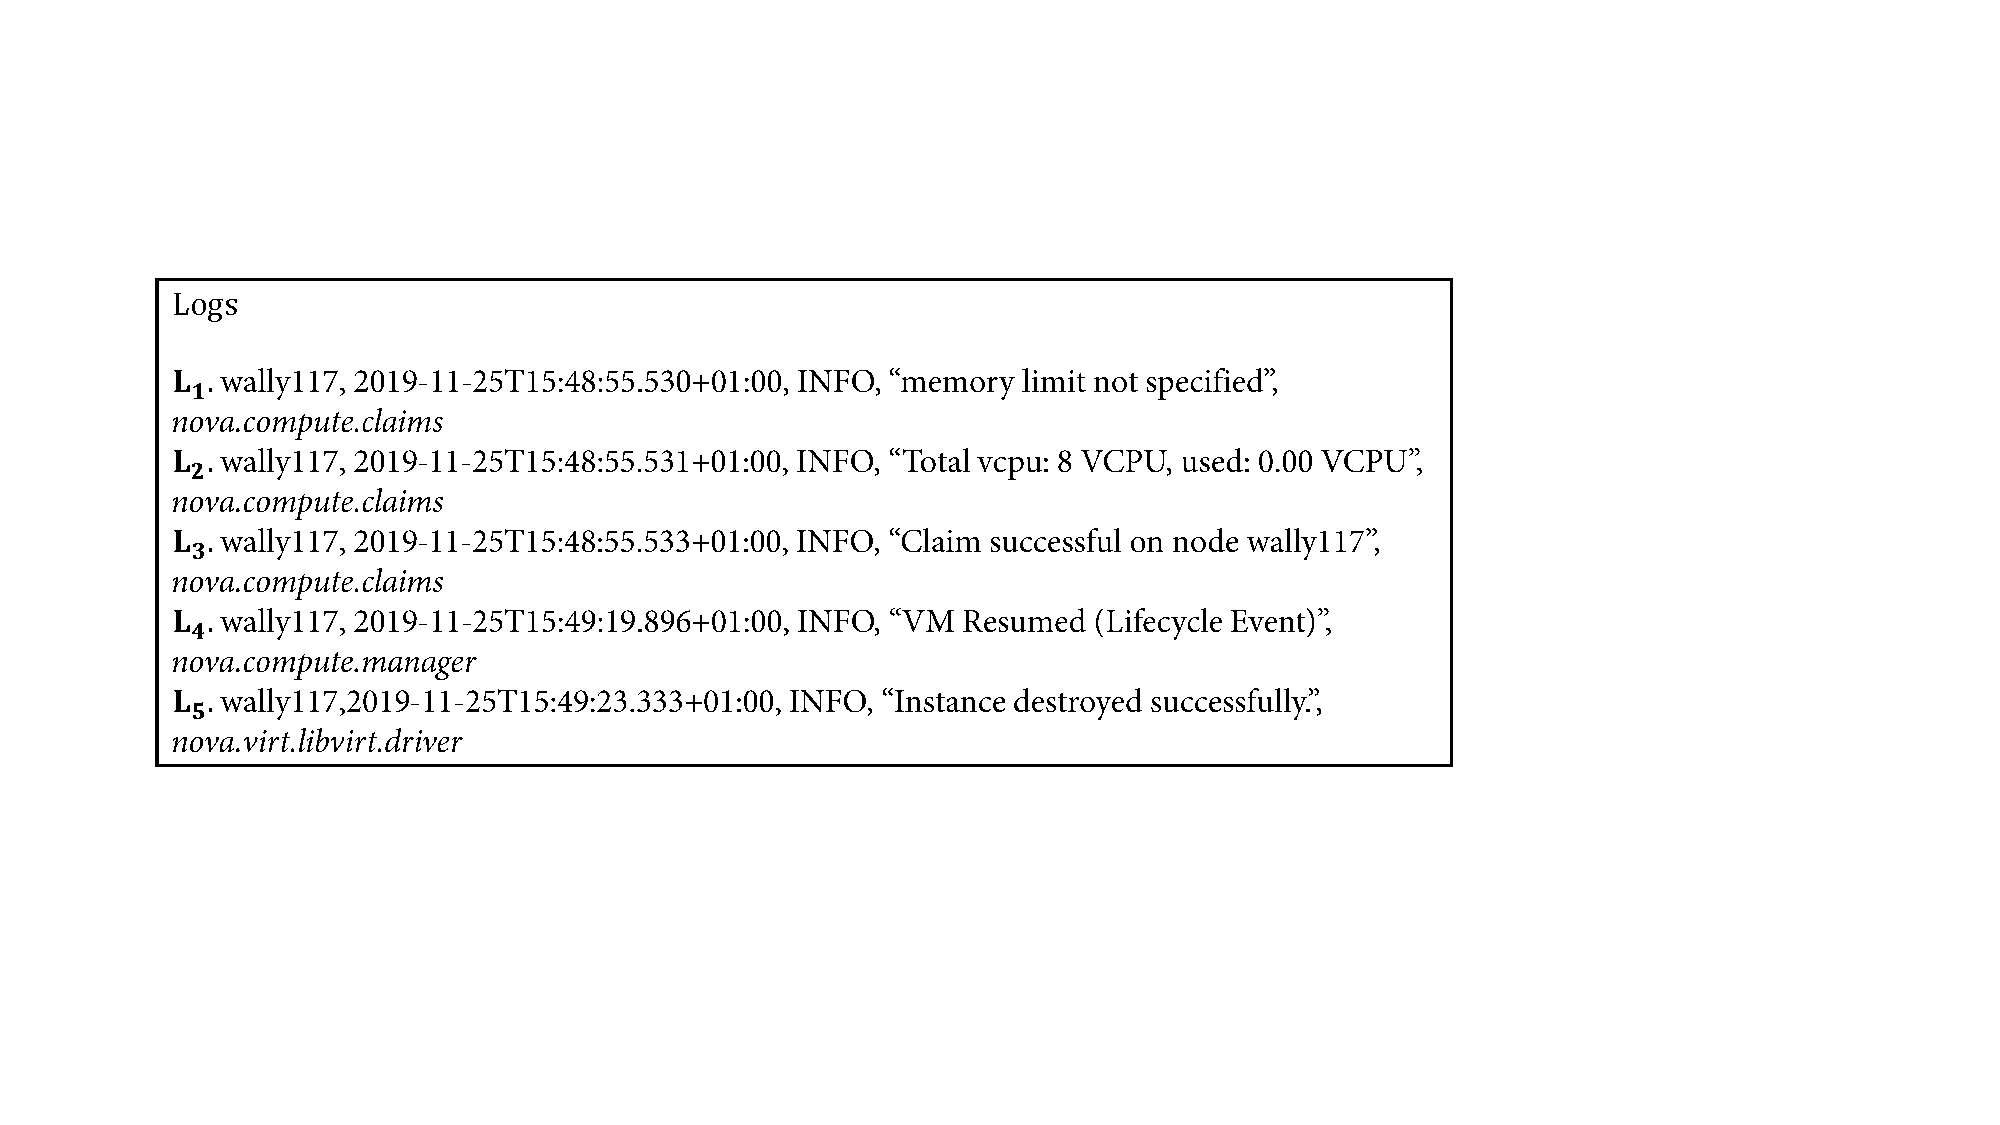
\includegraphics[width=1.0\textwidth]{gfx/chap2/log_lines.pdf}}
\caption{Raw log messages}
\label{fig:log_lines}
\end{figure}

Almost all live software systems have the property that the log statements from their services evolve and are prone to processing noise over time. In support of the evolving services property, a study from Microsoft~\cite{zhang2019robust} analyzed the behavior of one of their services in a distributed system over a period of one month. The total number of log messages increased from 2204 in version 1.0 of the service to 2763 in version 8.0 (latest version). The number of unchanged log events reduced drastically in the newer versions. In the latest version, the number of changed log events accounted for 30.3\% of the total log events. Moreover, processing noise is introduced during collection, retrieval, and pre-processing of log data, which are not truly anomalies of the system. For example, inaccurate log parsing can degrade the performance of an anomaly detection model~\cite{he2016evaluation}. He et al.~\cite{he2016evaluation} found that existing log parsers are not sufficiently accurate. More importantly, He, et al. also pointed out that log mining is sensitive to some critical events. They claimed that 4\% errors in parsing could even cause an order of magnitude performance degradation in anomaly detection (from 40\% to 3.7\%). In support of this study, Zhang et al.~\cite{zhang2019robust} found that most of the parsing errors are caused by missing/adding a few keywords from/into log events.  We note that to develop robust methods, these challenges must be directly addressed during the modeling process.

% In this thesis, we propose methods for log parsing and anomaly detection that aim to reduce the gap from the previously proposed methods to the desired goal that these approaches should be robust and generalize in such complex environments where the logs change.

\subsection{Traces}
Strong failures in complex distributed systems infrequently occur because of one particular event happening in one specific component of the system. Often, various possible triggers across a highly interconnected graph of components are involved. By solely observing discrete events that occurred in any given component at some point in time, it becomes hard to determine all such triggers. This the strongest drawback that log data face. To circumference this challenge, often postprocessing is needed to connect alarms from several log events and provide more insights. 

With the introduction of distributed tracing and traces as a representation of a series of causally related distributed events that encode the end-to-end request flow through a distributed system, the drawbacks of log data are addressed. Traces are a representation of logs, in other words, inter-connected logs; the data structure of traces looks almost like that of an event log. A single trace can provide visibility into the service response time to a request, the path traversed by a request as well as the structure of a request. The path of a request allows software developers and operators to understand the different services involved in the path of a request, and the structure of a request helps one understand the junctures and effects of asynchrony in the execution of a request. The response time is related to the actual user experience and the Quality of Service (QoS).

\begin{figure}[!t]
\centerline{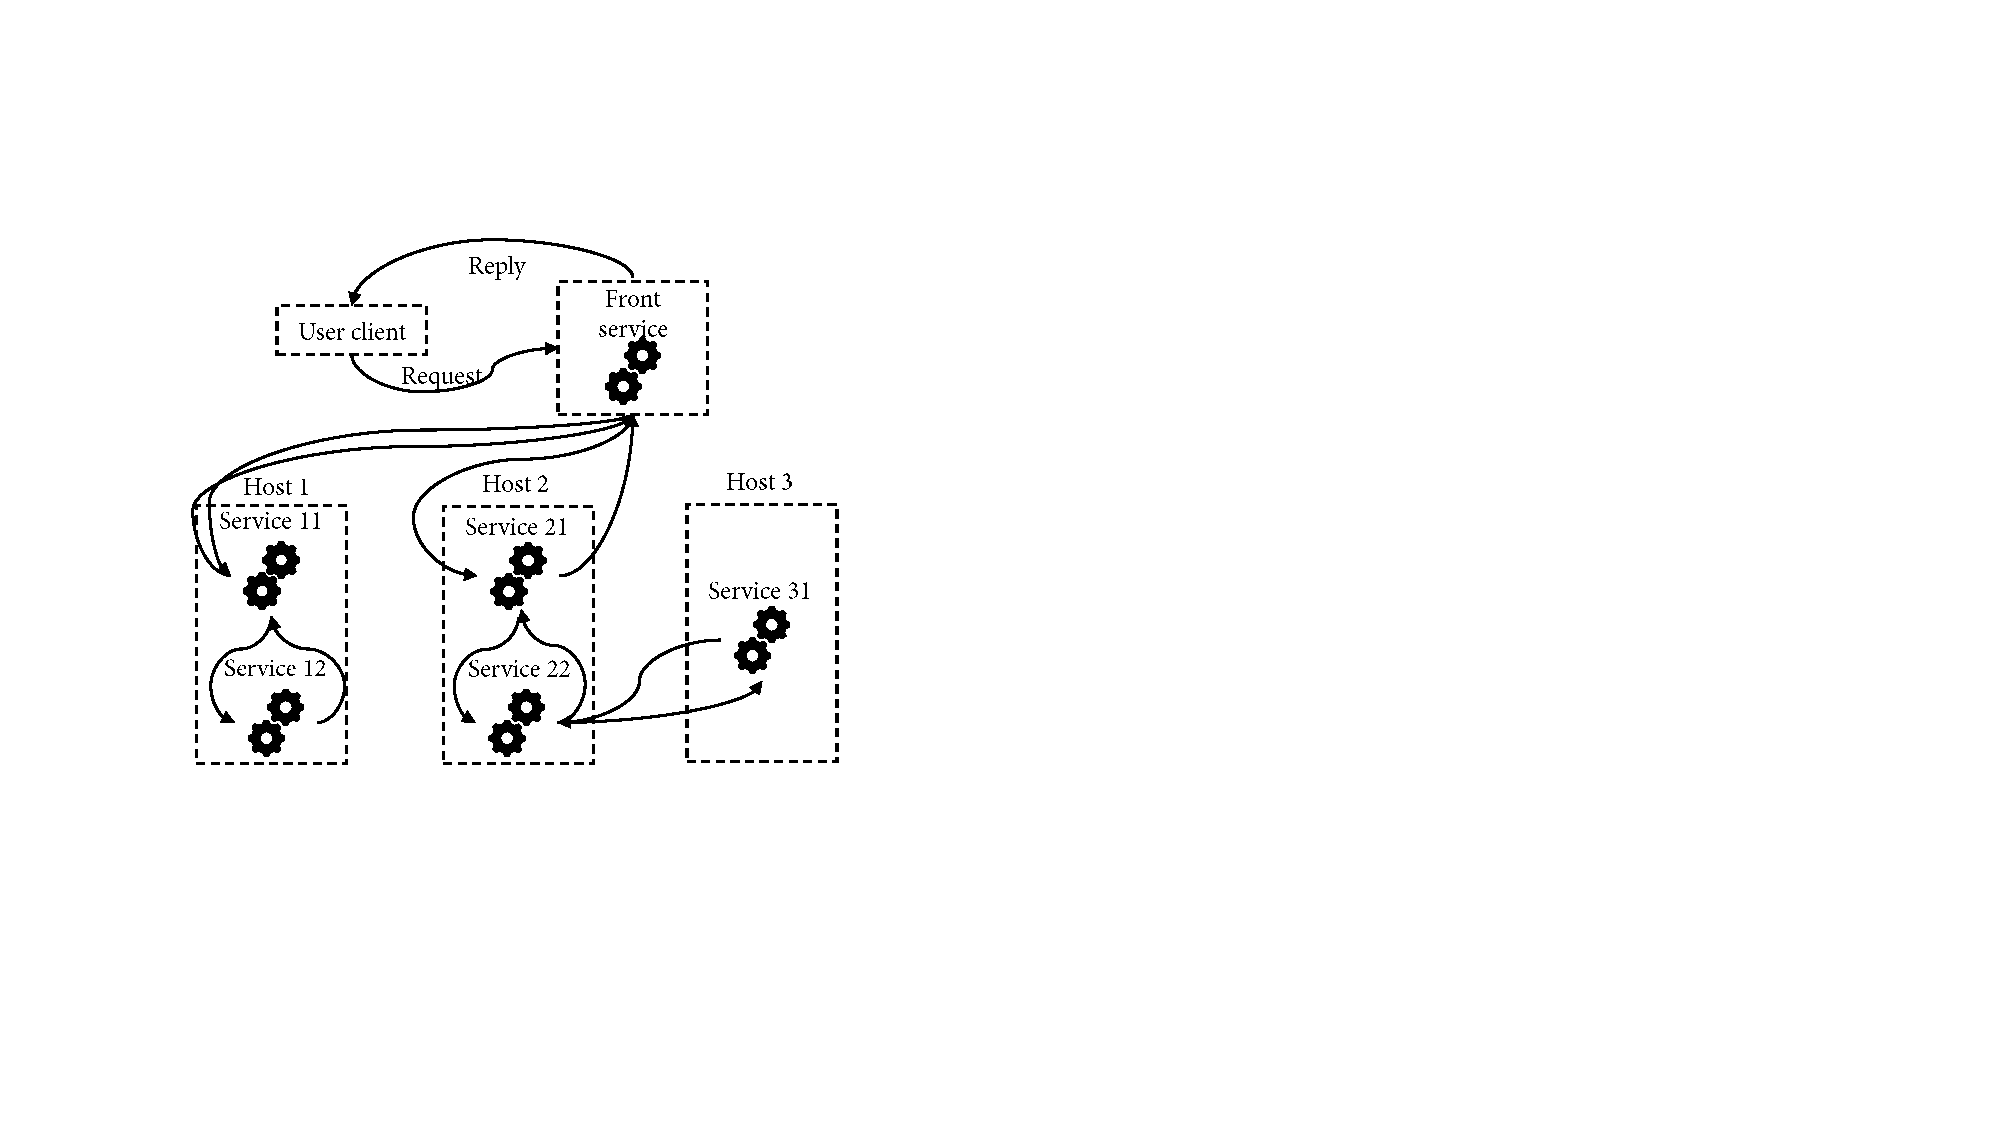
\includegraphics[width=0.8\textwidth]{gfx/chap2/pathmicroservice.pdf}}
\caption{Path taken through simple microservice system on behalf of the user request.}
\label{fig:pathmicroservice}
\end{figure}

A tracing infrastructure (e.g., Dapper~\cite{sigelman2010dapper}) for distributed services records information about all the work done in a system on behalf of a given initiator. In Figure~\ref{fig:pathmicroservice}, we show a system with 4 servers and 6 microservices. In following we describe the path of invocation of services and how a simple trace should look. A user sends a request at the front end, the front service sends two calls to microservices in host 1 and 2. Service 11 on host 1 calls service 12 (e.g., database) and responds to the request from the frontend, but service 21 and 22 require work from service 31 at host 3, before a reply is sent to the frontend. A simple trace for this request would be a collection of message identifiers and timestamped events for every message sent and received at each server.

\begin{figure}[htbp]
\centerline{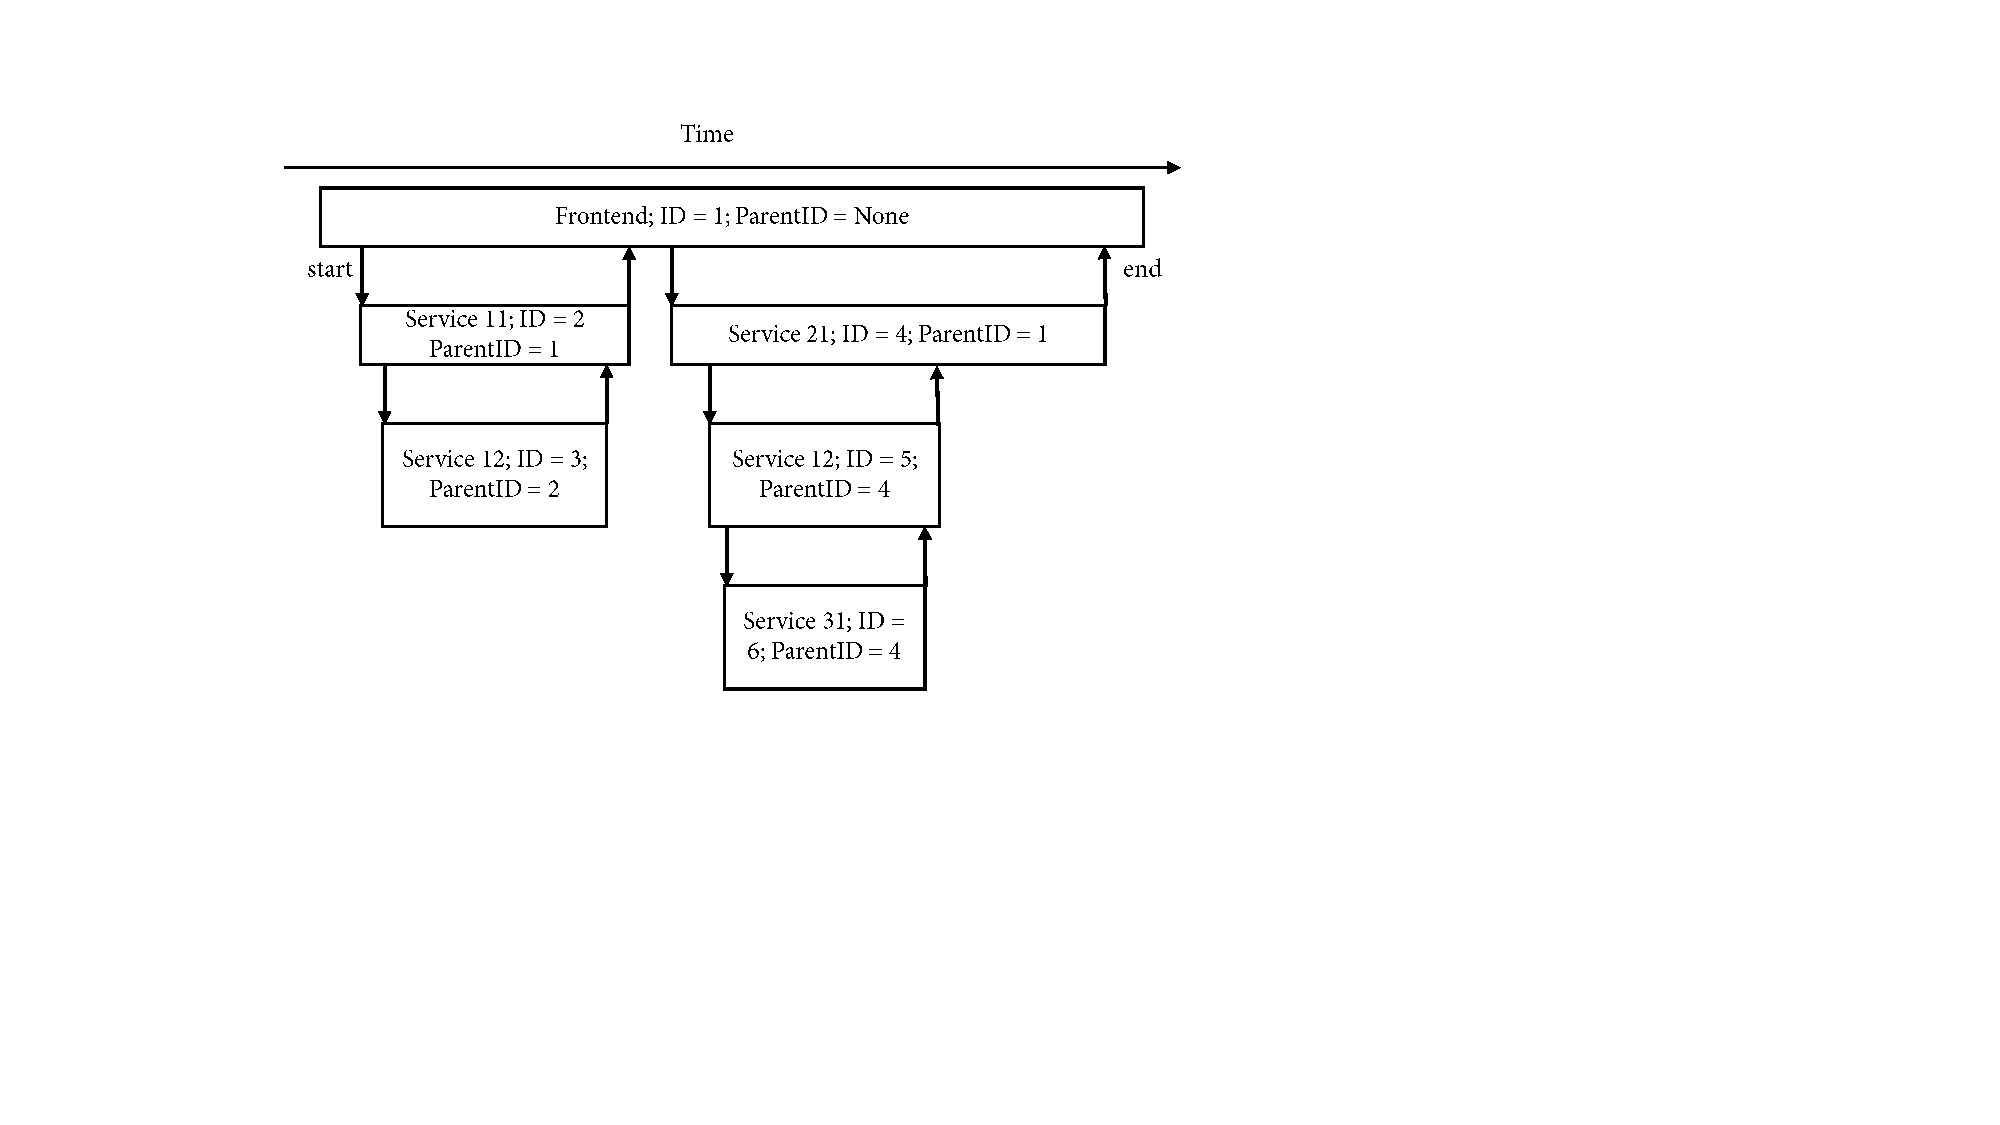
\includegraphics[width=0.8\textwidth]{gfx/chap2/temporal_relationship.pdf}}
\caption{The causal and temporal relationship between events.}
\label{fig:temporalevents}
\end{figure}

Such execution path with distributed tracing naturally can be described as a tree. In a trace tree, the tree nodes are basic units of work, which we refer to as events or spans. Each service invocation produces one span in the trace. The edges indicate a causal relationship between services. We illustrate how spans form the structure of a larger trace in Figure~\ref{fig:temporalevents}. Tracing records a human-readable span name for each span, as well as a Span ID and Parent ID. To reconstruct the causal relationships between the individual spans in a single distributed trace, we need to follow the parent--child relationship between the spans (representing a service invocation). Spans created without a Parent ID are known as root spans. All spans associated with a specific trace also share a common identifier Trace ID. All of these IDs are probabilistically unique 64-bit integers.

\begin{figure}[htbp]
\centerline{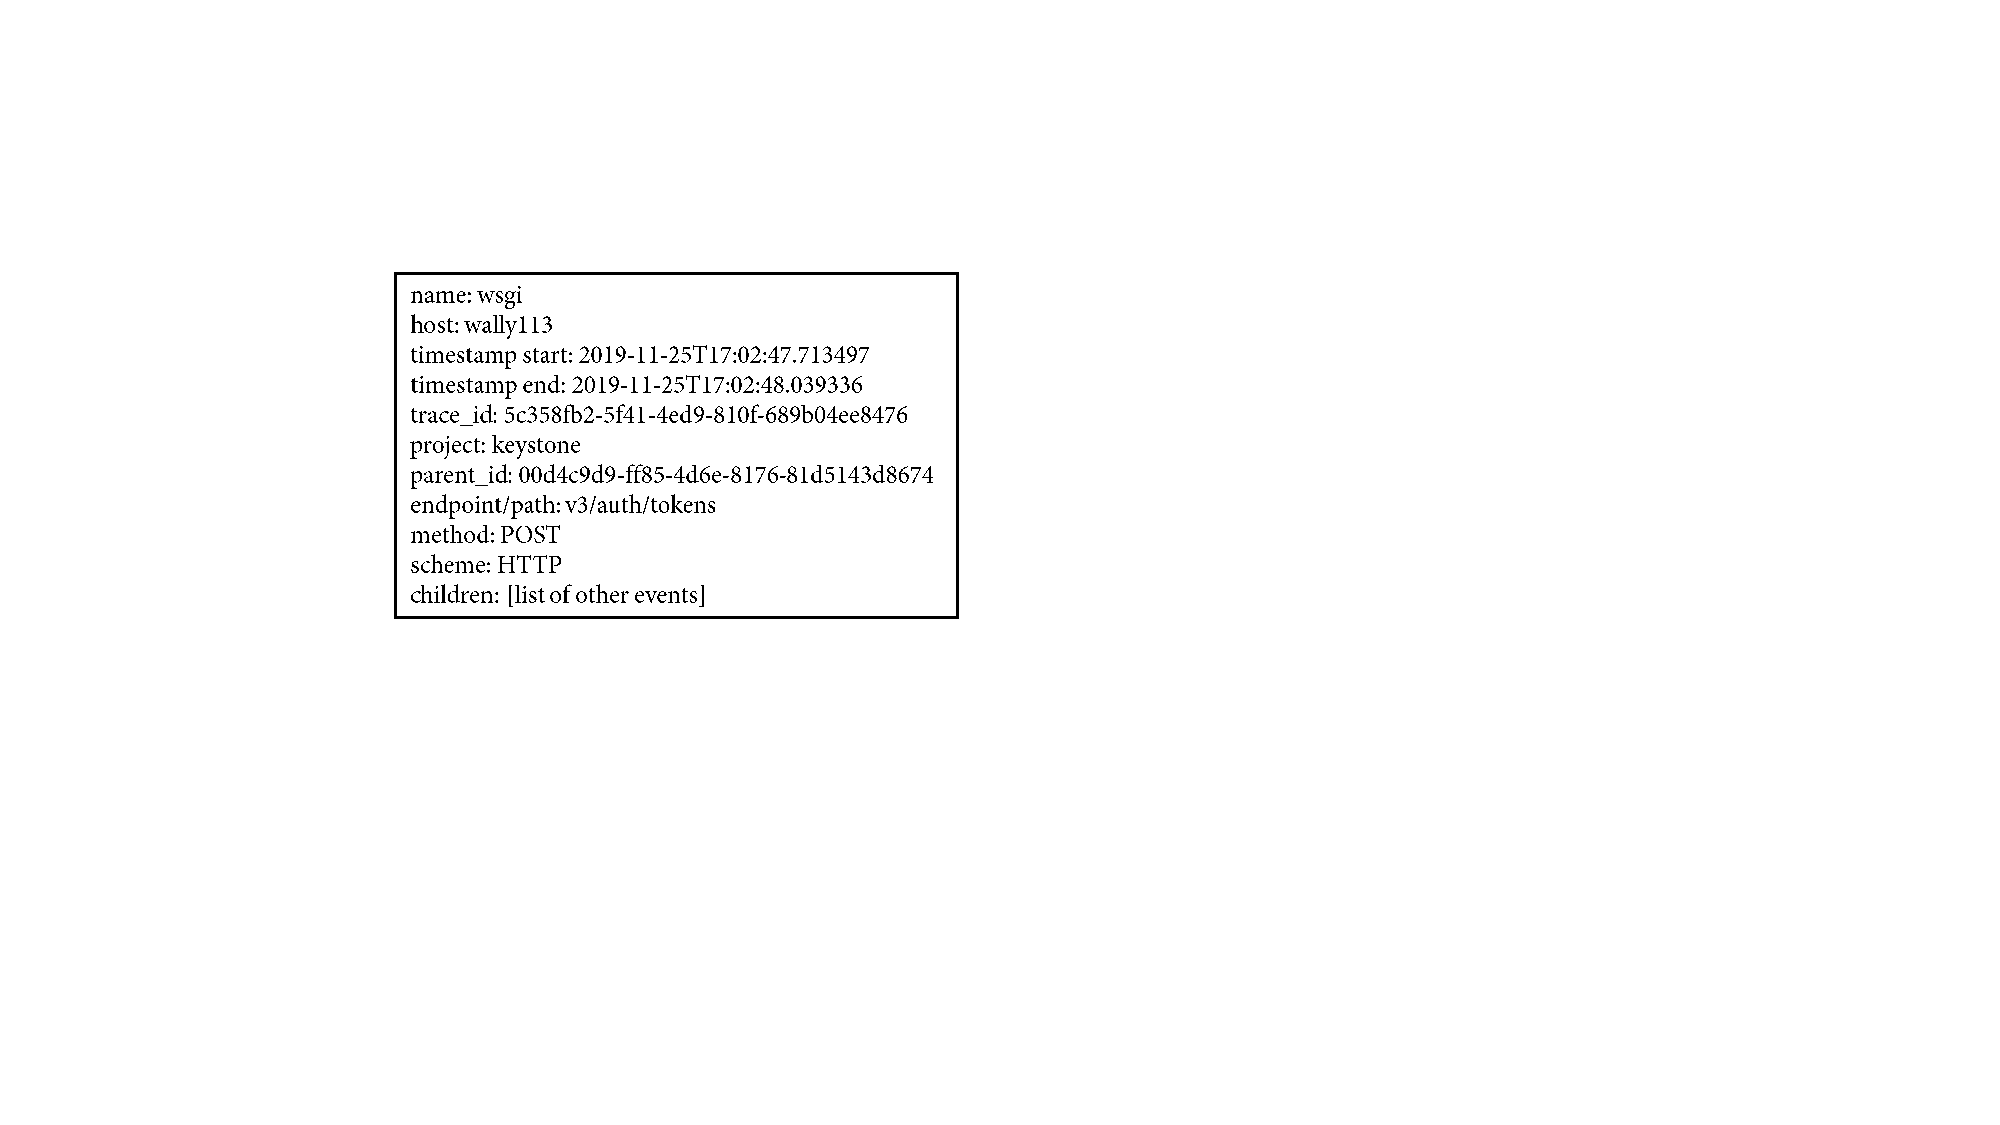
\includegraphics[width=0.8\textwidth]{gfx/chap2/single_event.pdf}}
\caption{A detailed view of a single event.}
\label{fig:singleevent}
\end{figure}

Figure~\ref{fig:singleevent} provides a more detailed view of the logged events in a typical trace span. As shown, each span within the trace is described by its start and stop time, name of the host on which the service is, name of the service/project, HTTP endpoint, and list of  its children spans/services. If application owners choose to augment the trace with their annotations, these are also recorded with the rest of the span data. 

Tracing data presents several challenges when it comes to analysis, learning, and concluding measurement noise due to highly complex environment, system overhead because in order tracing to be effective almost every component needs to be instrumented, variety of trace lengths~\cite{nedelkoski2019anomalymultimodal}, and similarly to the logs, constant evolution of the traces due to changes in the software. Therefore, similar challenges discussed in the previous section for logs hold for the traces as well.

\subsection{Metrics}
Most components of the software infrastructure serve as a resource to other systems. Some resources are low-level—for instance, a server resources include such physical components as CPU, memory, disks, and network interfaces. But a higher-level component, such as a database or a microservice, can also be considered a resource if another system requires that component to produce work. Resource metrics can help reconstruct a detailed picture of a system's state, making them valuable for investigation and diagnosis of problems. Often, for each resource in a system, several metrics are collected in key areas:
\begin{itemize}
    \item utilization is the percentage of time that the resource is busy or the percentage of the resource’s capacity that is in use.
    \item saturation is a measure of the amount of requested work that the resource cannot yet service, often queued.
    \item errors represent internal errors that may not be observable in the work the resource produces.
    \item availability represents the percentage of time that the resource responded to requests. This metric is only well-defined for resources that can be actively and regularly checked for availability.
\end{itemize}

We define a single observation of a metric as a value, a timestamp, and sometimes a series of properties that describe the observation, such as a source or tags. The combination of these data point observations is called a time series. Since metrics are just numbers measured over intervals of time, they can be compressed, stored, processed, and retrieved very efficiently. Metrics are optimized for storage and enable longer retention of data, which can in turn be used to build dashboards to reflect historical trends. Metrics allow for effective and valid aggregations (daily or weekly frequency). Metrics transfer and storage has a constant overhead. The cost of metrics does not increase in lockstep with user traffic or any other system activity. Metrics, once collected, are more malleable to mathematical and statistical transformations such as sampling, aggregation, summarization, and correlation, which make it better suited for monitoring and profiling purposes. Metrics are also better suited to trigger alerts, since running queries against an in-memory time-series database is far more efficient than running a query against a distributed system storage, and then aggregating the results before deciding if an alert needs to be triggered.

In metric data from a distributed system, several challenges arise, including the lack of labeled data, concept drift, and concept evolution. Other major sources of difficulties emerge due to the low signal-to-noise ratio, the presence of multiple frequencies and multiple distributions, the large number of distinct time series generated by microservice applications, and the presence of concept drifts. The signal-to-noise ratio is typically very low as many different components affect the response time of microservices such as switches, routers, memory capacity, CPU performance, programming languages, thread, and process concurrency, bugs, and volume of user requests. Multiple frequencies are correlated with system and user behavior since request patterns are different, e.g., from hour to hour due to business operation hours, from day to day due to system maintenance tasks, and from month to month due to cyclic patterns.


\subsection{Three cornerstones of observability}
Logs, metrics, and traces serve their unique purpose and are complementary. In unison, they provide maximum visibility into the behavior of distributed systems. Thus, these three types of data in distributed systems are a cornerstone for further analysis such as anomaly detection, which takes a central part in this thesis. In the following, we provide background knowledge for anomaly detection as a machine learning task.

\begin{figure}[!b]
\centerline{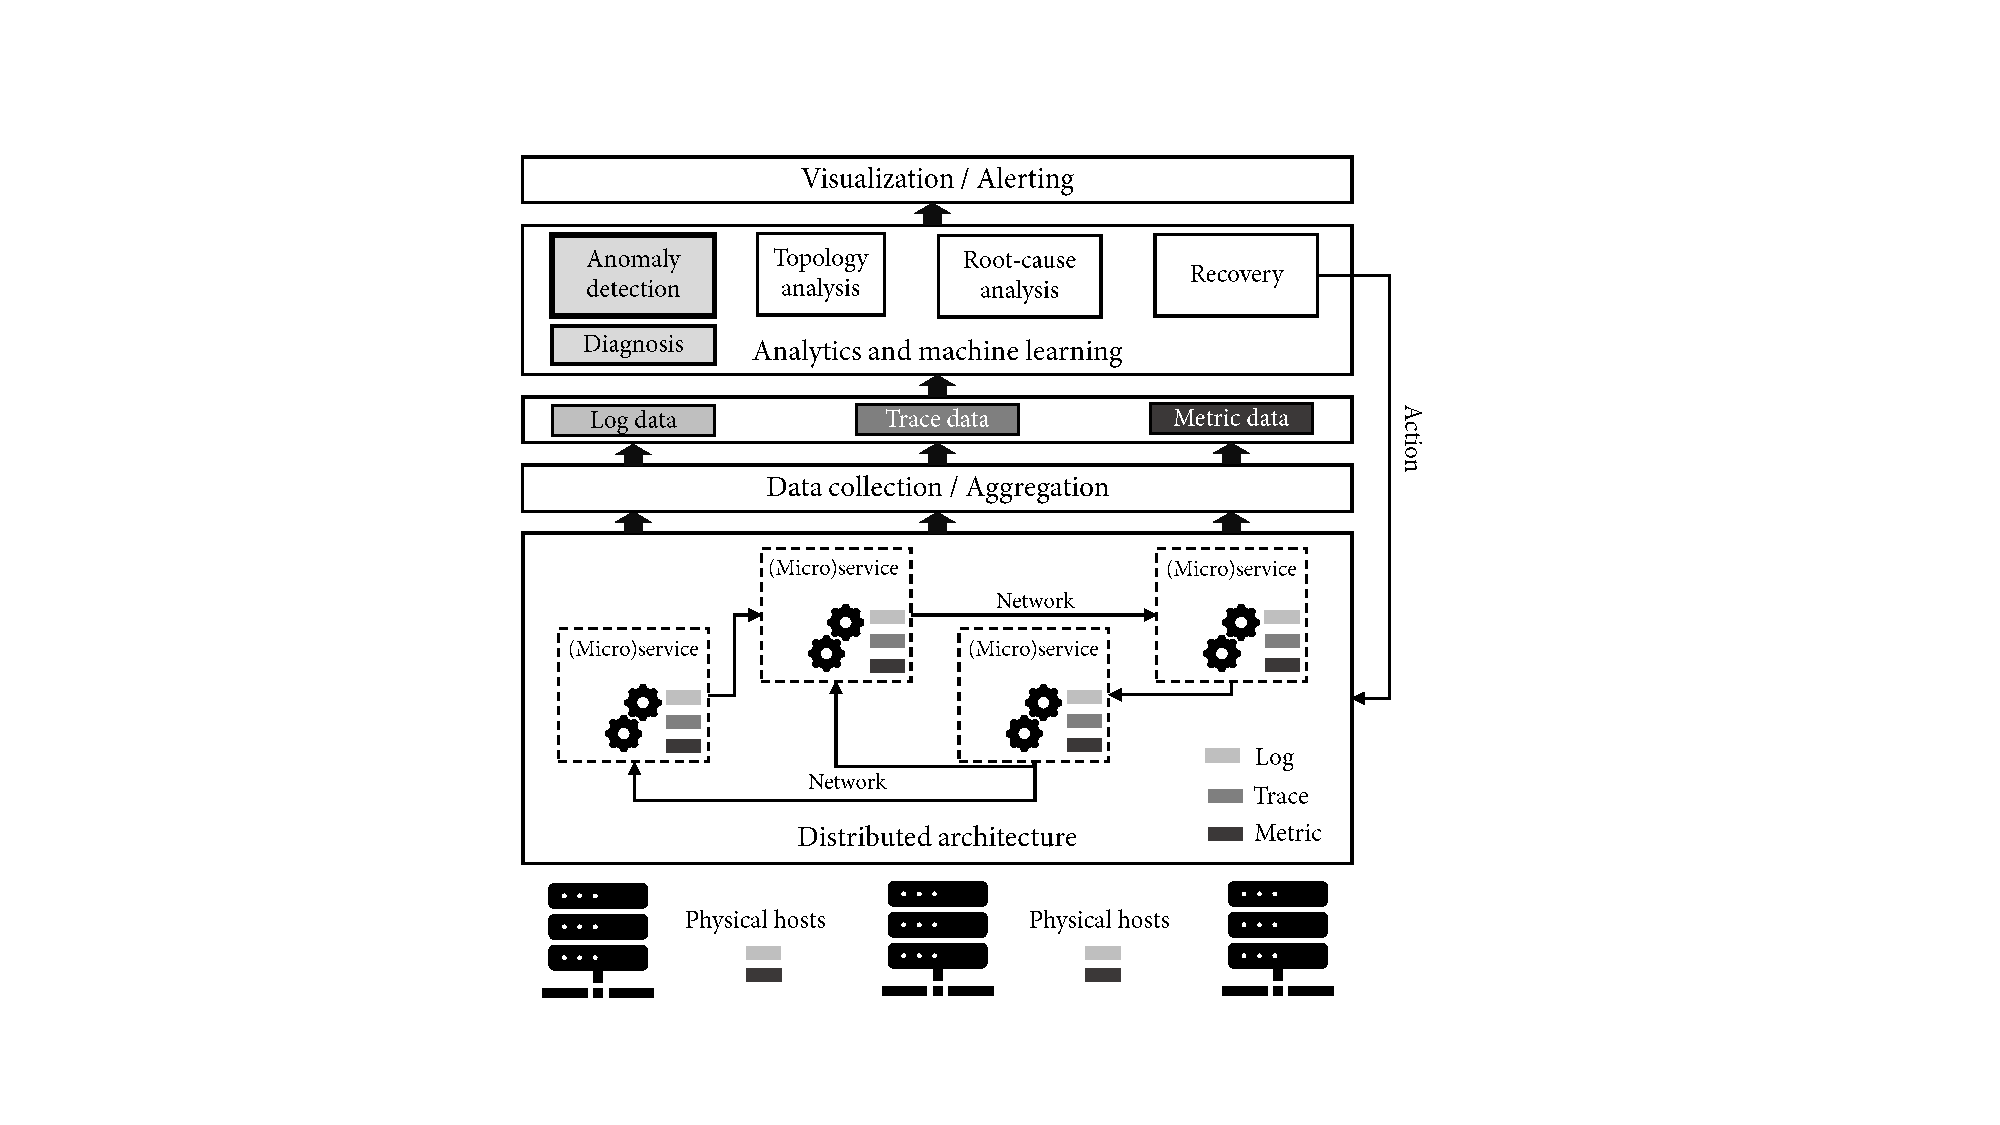
\includegraphics[scale=0.8]{gfx/chap2/aiopsplatform.pdf}}
\caption{Overall architecture of a distributed system with integrated observability components (logs, traces, and metrics). On top the data is analyzed and reported/visualized.}
\label{fig:aiopsplatform}
\end{figure}

\section{AIOPs: Reference Architecture}
In previous sections, we explained the need for observability in distributed systems and what are the major observability components. We noted that they are also basis for further system analysis including anomaly detection, root-cause analysis, debugging, and self-healing among others. In this section, we put the observability and the anomaly detection together in a broader context platform called Artificial Intelligence for IT operations (AIOPs platform). We show a reference architecture in Figure~\ref{fig:aiopsplatform}. AIOPs combines big data from the observability components and machine learning (e.g., anomaly detection) to replace a broad range of IT Operations tasks. In Figure~\ref{fig:aiopsplatform} a software based on a distributed architecture (e.g., microservices) is deployed on physical resources. In each of the physical hosts often metric and log data is collected. Similarly, in every (micro)service of the distributed system there are three data collection components: logs, traces, and metrics. The data is then aggregated and forwarded to the analytics part. For the metric data, the aggregation is done per service where metrics such as CPU, memory, disk utilization, and network statistics are collected. The logs from all services are aggregated in a database with a possible separation by service/physical host. Finally, the tracing data involves multiple hosts and services that are traversed while execution a request (e.g., user request). The data serves as basis for the analytics and machine learning part where several major tasks are performed. As one of the first tasks of troubleshooting and recovery is anomaly detection and fault diagnosis. The found anomalies together with the system topology are utilized by the root cause component to find the root cause of why the anomaly/fault happened. Lastly, in the recovery module takes the root cause and matches it with a possible recovery action which is executed to restore a failed component, or to prevent further fatalities. Finally, the alerts from the anomaly detection, the root cause and the recovery action are visualized to the developers, reliability engineers, and management teams to gain better insights on the system. 

In following we set the background knowledge in anomaly detection methods and other analytical concepts.

\section{Anomaly Detection}
Anomaly detection has been a lasting yet active research field in various research communities for several decades. As an application-driven research field, numerous methods have been proposed including in statistics, computer systems, healthcare, banking, and earth sciences~\cite{Aggarwal:2013:OA:2436823}. Anomaly detection is used as a general term for wide variety of techniques and approaches that share the common goal of finding unusual observations in a given data. A general definition that is widely accepted of what an anomaly is, was given by Hawkins~\cite{hawkins1980identification}:

\begin{center}
\textit{
"An outlier (anomaly) is an observation which deviates so much from
other observations as to arouse suspicions that it was generated by a
different mechanism."}
\end{center}

There have also been predecessors, e.g., by Grubbs in 1969~\cite{grubbs1969procedures}:

\begin{center}\textit{ 
"An outlying observation, or "outlier" (anomaly), is one that appears to deviate markedly from other members of the sample in which it occurs."}   
\end{center}

These definitions point out that anomaly detection is quite old field for computer science and statistics. However, the importance of anomaly detection increased significantly only recently with the appearance of the internet, online services, big data, large computer systems, and their corresponding economical impact. Today, practically all online services rely on a mix of anomaly detection methods. For example, cloud platforms utilize anomaly detection to improve their resilience and reliability, fraud detection is heavily used in the banking sector, and intrusion detection tools are implemented to prevent cyber attacks. Depending of the application and the context of use, the term "anomaly" is often substituted by outlier, exception, noise, abnormality, and deviations. 

A common anomaly detection approach is to define a region representing normal behavior and declare any observation in the data which does not belong to this normal region as an anomaly. However, several properties make this apparently simple approach very hard~\cite{chandola2009anomaly,pang2020deep}:
\begin{itemize}
    \item Defining a normal region which captures every possible normal behavior is very difficult due to the fact that knowing every possible normal behaviour is not possible in most applications.
    \item When anomalies are the result of malicious actions, the malicious adversaries often adapt themselves to make the anomalous observations appear like normal.
    \item In many domains normal behavior keeps evolving and a current notion of normal behavior might not be sufficiently representative in the future.
    \item Availability of labeled data for training/validation of models used by anomaly detection techniques is usually a major issue.
    \item Often the data contains noise which tends to be similar to the actual anomalies and hence is difficult to distinguish and remove.
\end{itemize}

The complex nature of the problem leads to number of detection challenges that still remain open in various applications.

\begin{enumerate}
    \item \textbf{Low prediction rate.} Anomalies are highly rare events and it is difficult to identify all of them. Many normal instances are wrongly reported as anomalies while sophisticated anomalies are missed. Plethora of research have been introduced over the years~\cite{liu2008isolation,breunig2000lof}, however, still there is a high number false positives on real-world datasets~\cite{du2017deeplog,campos2016evaluation}. 
    \item \textbf{Anomaly detection in high-dimensional and not conditional data.} Anomalies often exhibit evident abnormal characteristics in a low-dimensional space yet become hidden and unnoticeable in a high-dimensional space. However, identifying high-order, nonlinear and heterogeneous feature interactions and couplings may be essential in high-dimensional data yet remains a major challenge for anomaly detection. Also, it is challenging to detect anomalies from instances that may be dependent on each other such as by temporal, spatial, graph-based and other inter-dependency relationships~\cite{pang2020deep}.
    \item \textbf{Anomaly detection from noisy data.} Many anomaly detection methods assume the given labeled training data is clean, which can be highly vulnerable to noisy instances that are mistakenly labeled as an opposite class label. For example, in a training data collected from a computer system, as labels are not available, often is assumed that all the data is normal. However, most probably there are anomaly samples in the training data, which can contaminate and degrade the model performance. Therefore, the main challenge is how to build models robust to such not known deviations. 
    \item \textbf{Detection of complex anomalies.} One main challenge  is to incorporate the concept of conditional/group anomalies into anomaly measures/models. Also, current methods mainly focus on detect anomalies from single data sources, while many applications require the detection of anomalies with multiple heterogeneous data sources. One main challenge is that some anomalies can be detected only when considering two or more data sources.
\end{enumerate}

Due to the above challenges, the anomaly detection problem, in its most general form, is not easy to solve. In fact, most of the existing anomaly detection techniques solve a specific formulation of the problem that is application-dependent. In distributed system data such as the logs, traces, and metrics, similar challenges arise. For example, defining normal regions that captures all normal system behaviour is not possible as large distributed systems such as the cloud are constantly prone to new infrastructure and software updates, varying levels of load, noise, and users. For the same reason, the data keeps evolving where the current normal behaviour may be outdated in future. Malicious attacks on the large-scale service providers are increasingly sophisticated and hard to detect as they emulate normal behaviours~\cite{yan2015software}. Logs and traces are often mixture of textual and numeric data that requires joint analysis for successful anomaly detection. Both are high-dimensional and complex data. Moreover, often in the collected training data there is high level of noise due to the complex nature of the system and possible corruptions/inclusion of anomalies. 

\subsection{Types of anomalies}

Anomalies appear in many different forms and context. In general, regarding the type of anomalies that could possibly arise, three different types are considered (Figure~\ref{fig:typesofanomalies}):
\begin{itemize}
%Give examples in system data
    \item \textbf{Point anomalies} are data points that appear isolated from the bulk of the data.
    \item \textbf{Contextual anomalies}, sometimes also called conditional anomalies, are data points whose values itself are only anomalous in a specific contextual relation. Contextual features might be time, location, or a broader data structure.
    \item \textbf{Collective anomalies} consist of a sequence of data points that only as a group, and not as individual points, can be tagged anomalous.
\end{itemize}

\begin{figure}[htbp]
\centerline{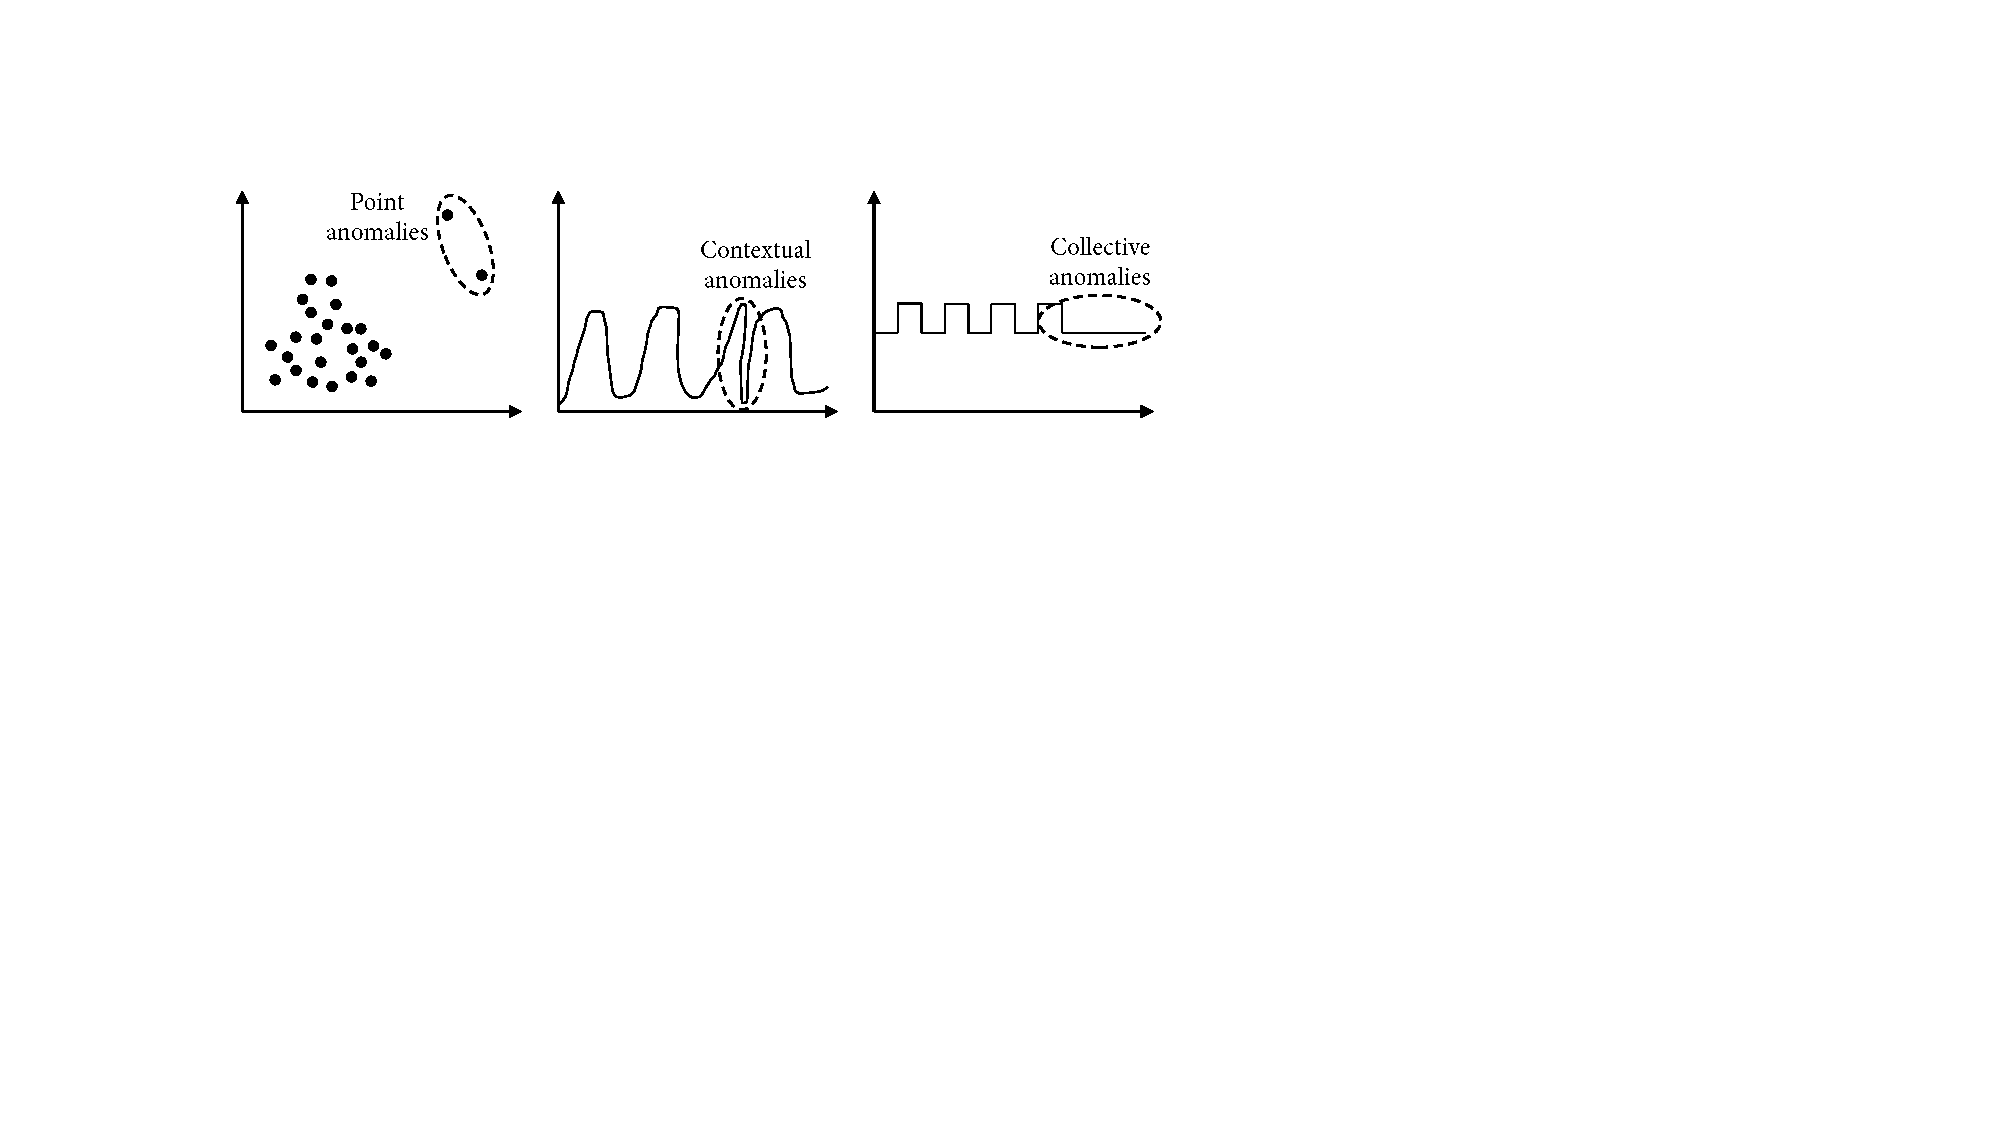
\includegraphics[width=1.0\textwidth]{gfx/chap2/typesofanomalies.pdf}}
\caption{An example of point anomalies (left); an example of a contextual anomaly (middle, note that the value of the data instance at the minimum are not anomalous, but in the context where the dashed line is it is); an example of a collective anomaly (right), the absence of a whole group at of data points forms an anomaly.}
\label{fig:typesofanomalies}
\end{figure}

Point anomalies have been focus of the research more extensively and many methods readily assume that data points come as independent instances. If, however, data exhibits strong dependency structure, handling data points as independent instance might not suffice anymore and therefore contextual and collective anomalies are considered. 

The labels associated with a data instance denote if that instance is normal or anomalous. It should be noted that obtaining labeled data which is accurate as well as representative of all types of behaviors, is often prohibitively costly. Labeling in all domains is often done manually by a human expert and hence requires substantial effort to obtain the labeled training data set. Typically, getting a labeled set of anomalous data instances which cover all possible type of anomalous behavior is more difficult than getting labels for normal behavior. Moreover, the anomalous behavior is often dynamic in nature, e.g., new types of anomalies might arise, for which there is no labeled training data. In certain cases, such as air traffic safety, anomalous instances would translate to catastrophic events, and hence will be very rare. The provision of labeled data from distributed systems is costly and challenging owing mostly to practical limitations. As already mentioned, such systems undergo constant changes, e.g., software updates and hardware modernization, where labeled data become deprecated over time. Moreover, injections of anomalies to obtain data points is not possible as most running systems can not take the risk of possible downtimes. Based on the extent to which the labels are available, anomaly detection techniques can operate in one of the following three modes: supervised, semi-supervised, and unsupervised anomaly detection, which we discuss in following.

\subsection{Supervised anomaly detection}
Methods for supervised anomaly detection are similar to building predictive models. These techniques assume the availability of a training data set which has labeled instances for normal as well as anomaly class. Typical approach in such cases is to build a predictive model for normal against anomaly classes~\cite{chandola2009anomaly}. Any unseen data instance is compared against the model to determine which class it belongs to. There are two major issues that arise in supervised anomaly detection. First, the anomalous instances are far fewer compared to the normal instances in the training data. Issues that arise due to imbalanced class distributions have been addressed in the data mining and machine learning literature. Second, obtaining accurate and representative labels, especially for the anomaly class is usually challenging. A number of techniques have been proposed that inject artificial anomalies in a normal data set to obtain a labeled training data set~\cite{theiler2003resampling, steinwart2005classification}. However, as labeled data from a distributed system is prohibitively costly, we do not directly address this category in this thesis.

\subsection{Semi-supervised anomaly detection}
In many real-world applications one may also have access to some verified (i.e., labeled) normal or anomalous samples in addition to the unlabeled data. Such samples could be hand labeled by a domain expert for instance. This leads to a semi-supervised anomaly detection problem: given $n$ (mostly normal but possibly containing some anomalous contamination) unlabeled samples $x_1,\dots, x_n$ and $m$ labeled samples $(\hat{x_1}, \hat{y_1}),\dots,(\hat{x_m}, \hat{y_m})$, where $\hat{y} = 0$ and $\hat{y} = 1$ denote normal and anomalous samples respectively, the task is to learn a model that compactly characterizes the normal class.

The term semi-supervised anomaly detection has been used to describe two different anomaly detection settings. Most existing semi-supervised AD methods, both shallow and deep only incorporate the use of labeled normal samples but not labeled anomalies, i.e. they are more precisely instances of Learning from Positive (i.e., normal) and Unlabeled Examples (LPUE). A few works have investigated the general semi-supervised AD setting where one also utilizes labeled anomalies, however existing deep approaches are domain or data-type specific~\cite{ruff2019deep,chandola2009anomaly}.

Since they do not require labels for the anomaly class, they are more widely applicable than supervised techniques. The typical approach used in such techniques is to build a model for the class corresponding to normal behavior, and use the model to identify anomalies in the test data. A limited set of anomaly detection techniques exist that assume availability of only the anomaly instances for training. Such techniques are not commonly used, primarily because it is difficult to obtain a training data set which covers every possible anomalous behavior that can occur in the data~\cite{ruff2019deep}.

\subsection{Unsupervised anomaly detection}
Techniques that operate in unsupervised mode do not require labeled training data, and thus are most widely applicable. The techniques in this category make the implicit assumption that normal instances are far more frequent than anomalies in the test data. If this assumption is not true then such techniques suffer from high false alarm rate. Many semi-supervised techniques can be adapted to operate in an unsupervised mode by using a sample of the unlabeled data set as training data. Such adaptation assumes that the test data contains very few anomalies and the model learnt during training is robust to these few anomalies. As this is the most practical learning scenario for anomaly detection, all proposed methods in this thesis belong to this category.

\subsection{Deep Anomaly Detection}
The performance of traditional algorithms in detecting outliers is sub-optimal on the sequence and image datasets since it fails to capture complex patterns in the data. In addition, there is need for large-scale anomaly detection: As the volume of data increases let us say to gigabytes then, it becomes nearly impossible for the traditional methods to scale to such large scale data to find outliers.

In recent years, deep learning has shown tremendous capabilities in learning expressive representations of complex data such as high-dimensional data, temporal data, spatial data and graph data, pushing the boundaries of different learning tasks. Deep learning for anomaly detection, deep anomaly detection for short, aim at learning feature representations or anomaly scores via neural networks for the sake of anomaly detection. In recent years, a large number of deep anomaly detection methods have been introduced, demonstrating significantly better performance than conventional anomaly detection on addressing challenging detection problems in a variety of real-world applications~\cite{pang2020deep}. However, the boundary between normal and anomalous (erroneous) behavior is often not precisely defined in several data domains and is continually evolving. This lack of well-defined representative normal boundary poses challenges for both conventional and deep learning-based algorithms.

Deep neural networks leverage complex compositions of linear/non-linear functions that can be represented by a computational graph to learn expressive representations~\cite{Goodfellow-et-al-2016}. Two basic building blocks of deep learning are activation functions and layers. Activation functions determine the output of computational graph nodes (i.e., neurons in neural networks) given some inputs. They can be linear or non-linear functions. Some popular activation functions include linear, sigmoid, tanh, ReLU (Rectified Linear Unit) and its variants. A layer in neural networks refers to a set of neurons stacked in some forms. Commonly-used layers include fully connected, convolutional \& pooling, and recurrent layers. These layers can be leveraged to build different popular neural networks. For example, multilayer perceptron (MLP) networks are composed by fully connected layers, convolutional neural networks (CNN) are featured by varying groups of convolutional \& pooling layers, and recurrent neural networks (RNN), \eg, vanilla RNN, gated recurrent units (GRU) and long short term memory (LSTM), are built upon recurrent layers. We refer the reader to Goodfellow et al.~\cite{Goodfellow-et-al-2016} for detailed description of the neural networks.

Given a dataset $\mathcal{X} =\{\mathbf{x_1}, \mathbf{x_2}, \cdots, \mathbf{x_N}\}$ with $\mathbf{x_i} \in \mathbb{R}^{D}$, let $\mathcal{Z} \in \mathbb{R}^{K}$ be a representation space, then deep anomaly detection aims at learning a feature representation mapping function $\phi(\cdot): \mathcal{X} \mapsto \mathcal{Z}$ or an anomaly score learning function $\tau(\cdot):\mathcal{X} \mapsto \mathbb{R}$ in a way that anomalies can be easily differentiated from the normal data instances in the $\phi$ or $\tau$ space, where both $\phi$ and $\tau$ are a neural network-enabled mapping function with $H \in \mathbb{N}$ hidden layers and their weight matrices $\Theta=\{\mathbf{M}^{1}, \mathbf{M}^{2}, \cdots, \mathbf{M}^{H}\}$. In the case of learning the feature mapping $\phi(\cdot)$, an additional step is required to calculate the anomaly score of each data instance in the new representation space, while $\tau(\cdot)$ can directly infer the anomaly scores with raw data inputs. 

Pang et al.~\cite{pang2020deep} provide an exhaustive overview of deep anomaly detection methods where the methods are grouped in three conceptual paradigms Deep Learning for Feature Extraction, Learning Feature Representations of Normality, and End-to-end Anomaly Score Learning. In following we discuss the main concepts and methods for each group, while for the details we refer the reader to more comprehensive reviews of the literature~\cite{pang2020deep,chalapathy2019deep}.

\subsubsection{Deep learning for feature extraction}
This category of studies represents the most basic application of deep learning techniques to anomaly detection. It aims at leveraging deep learning to extract low-dimensional feature representations from high-dimensional and/or non-linearly separable data for downstream anomaly detection. The feature extraction and the anomaly scoring are fully disjointed and independent from each other. Thus, the deep learning components work purely as dimensionality reduction only.  Formally, the approach can be represented as
\begin{equation}\label{eqn:featureextraction}
\centering
    \mathbf{z} = \phi(\mathbf{x}; \Theta),
\end{equation}

where $\phi:\mathcal{X} \mapsto \mathcal{Z}$ is a deep neural network-based feature mapping function, with $\mathcal{X}\in \mathbb{R}^{D}$, $\mathcal{Z} \in \mathbb{R}^{K}$ and normally $D \gg K$. An anomaly scoring method $f$ that has no connection to the feature mapping $\phi$ is then applied onto the new space to calculate anomaly scores.

Compared to the dimension reduction methods that are popular in anomaly detection, such as principal component analysis (PCA)~\cite{jolliffe2016principal}, deep learning techniques have been demonstrating substantially better capability in extracting semantic-rich features and non-linear feature relations~\cite{bengio2013representation,Goodfellow-et-al-2016}.

The accuracy of the anomaly detection in this case largely depends on the feature representations extracted by deep learning models, where they need to preserve the information that helps separate anomalies from normal instances.

\subsection{Learning feature representations of normality}
This section reviews the models from the perspective of normality learning. The deep anomaly detection methods in this category couple feature learning with anomaly scoring in some ways, which are different from the methods in the last section that fully decouple these two modules. 

This category of methods learns the representations of data instances by optimizing a generic feature learning objective function that is not primarily designed for anomaly detection, but the learned representations can still empower the anomaly detection since they are forced to capture some key underlying data regularities. Formally, this framework can be represented as

\begin{gather}
    \{\Theta^*, \mathbf{W}^*\} = \argmin_{\Theta,\ \mathbf{W}} \sum_{\xvec \in \mathcal{X}}\ell\Big(\psi\big(\phi(\mathbf{x};\Theta);\mathbf{W}\big)\Big) \label{eqn:genericfeature1},\\
    s_{\mathbf{x}} = f(\mathbf{x}, \phi_{\Theta^*}, \psi_{\mathbf{W}^*}) \label{eqn:genericfeature2},
\end{gather}

where $\phi$ maps the original data onto the representation space $\mathcal{Z}$, $\psi$ parameterized by $\mathbf{W}$ is a surrogate learning task that operates on the $\mathcal{Z}$ space and is dedicated to enforcing the learning of underlying data regularities, $\ell$ is a loss function relative to the underlying modeling approach, and $f$ is an anomaly scoring function that utilizes these two functions with the trained parameters $\Theta^*$ and $\mathbf{W}^*$ to calculate the anomaly score $s$.

This approach include methods that are driven by several perspectives, including data reconstruction, generative modeling, predictability modeling and self-supervised classification.

\subsubsection{Autoencoders}
This type of approach aims to learn some low-dimensional feature representation space on which the given data instances can be well reconstructed. This is a widely-used technique for data compression or dimension reduction~\cite{hinton2006ae,jiang2014dimensionalityreductionae,theis2017dimensionalityreductionae}. The heuristic for using this technique in anomaly detection is that the learned feature representations are enforced to learn important regularities of the data to minimize reconstruction errors; anomalies are difficult to be reconstructed from the resulting representations and thus have large reconstruction errors.

The assumtion is that normal data instances can be better restructured from compressed feature space than anomalies.

\begin{figure}[htbp]
\centerline{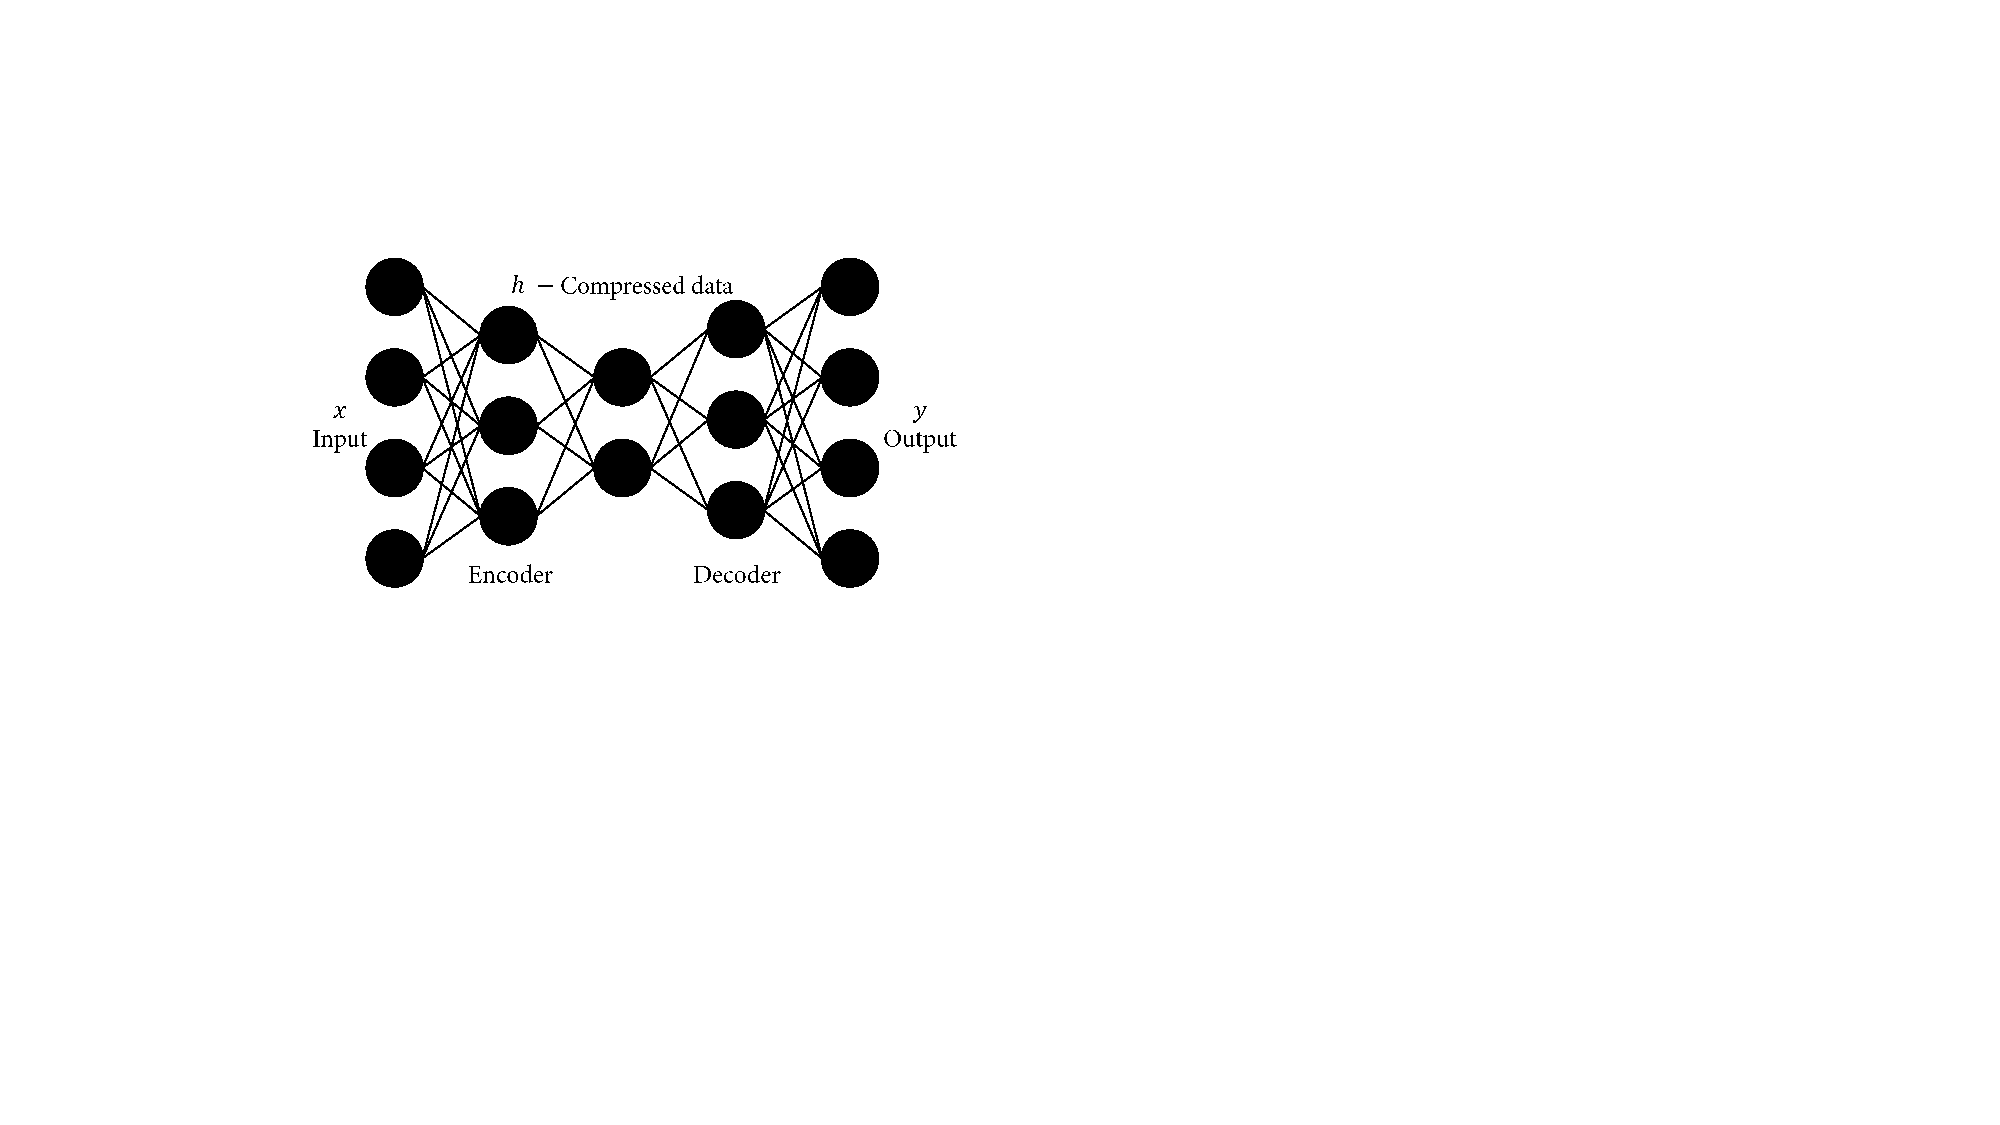
\includegraphics[scale=1.0]{gfx/chap2/autoencoder.pdf}}
\caption{Architecture of Undercomplete Autoencoder}
\label{fig:autoencoder}
\end{figure}

Autoencoder (AE) networks are the most commonly-used techniques in this category. An AE is composed of an encoding network and an decoding network. The encoder maps the original data onto low-dimensional feature space, while the decoder attempts to recover the data from the projected low-dimensional space. The parameters of these two networks are learned with a reconstruction loss function. A bottleneck network architecture (Figure~\ref{fig:autoencoder}) is often used to obtain low-dimensional representations than the original data, which forces the model to retain the information that is important in reconstructing the data instances. To minimize the overall reconstruction error, the retained information is required to be as much relevant as possible to the dominant instances, e.g., the normal instances. As a result, the data instances such as anomalies which deviate from the majority of the data are poorly reconstructed. The data reconstruction error therefore well fits the anomaly score. The basic formulation of this approach is given as follows.
\begin{gather}\label{eqn:ae}
    \mathbf{z} = \phi_e(\mathbf{x}; \Theta_e),\\
    \hat{\mathbf{x}} = \phi_d(\mathbf{z}; \Theta_d),\\
   \{\Theta_e^*, \Theta_d^*\} = \argmin_{\Theta_e,\Theta_d} \sum_{\xvec \in \mathcal{X}}\big\|\mathbf{x}-\phi_d\big(\phi_e(\mathbf{x};\Theta_e); \Theta_d\big)\big\|^2,\\
    s_{\mathbf{x}} = \big\|\xvec - \phi_d\big(\phi_e(\mathbf{x};\Theta_e^*); \Theta_d^*\big)\big\|^2,
\end{gather}
where $\phi_e$ is the encoding network with the parameters $\Theta_e$ and $\phi_d$ is the decoding network with the parameters $\Theta_d$. The encoder and the decoder can share the same weight parameters to reduce parameters and regularize the learning. $s_{\mathbf{x}}$ is a reconstruction error-based anomaly score of $\mathbf{x}$.

% Several types of regularized autoencoders have been introduced to learn richer and more expressive feature representations \cite{makhzani2014sparseae,vincent2010denoisingae,rifai2011contractiveae,doersch2016variationalae}. Particularly, sparse AE is trained in a way that encourages sparsity in the activation units of the hidden layer, \eg, by keeping the top-$K$ most active units \cite{makhzani2014sparseae}. Denoising AE \cite{vincent2010denoisingae} aims at learning representations that are robust to small variations by learning to reconstruct data from some predefined corrupted data instances rather than original data. Contractive AE \cite{rifai2011contractiveae} takes a step further to learn feature representations that are robust to small variations of the instances around their neighbors, which is achieved by adding a penalty term based on the Frobenius norm of the Jacobian matrix of the encoder's activations. Variational AE \cite{doersch2016variationalae} instead introduces regularization into the representation space by encoding data instances using a prior distribution over the latent space, preventing overfitting and ensuring some good properties of the learned space for enabling generation of meaningful data instances.

% As such, AEs are also widely leveraged to detect anomalies in data other than tabular data, such as sequence data \cite{lu2017sequenceae}, graph data \cite{ding2019graphae} and image/video data \cite{xu2015videoae}. In general, there are two types of adaptions of AEs to those complex data. The most straightforward way is to follow the same procedure as the conventional use of AEs with the exception that a particular network architecture tailored for a specific type of data is required to learn effective low-dimensional feature representations, such as CNN-AE \cite{hasan2016convae,zhang2019convolutionalae}, LSTM-AE \cite{malhotra2016lstmae}, Conv-LSTM-AE \cite{luo2017convolutionlstmae} and GCN (graph convolutional network)-AE \cite{ding2019graphae}. This type of AEs embeds the encoder-decoder scheme into the full procedure of these methods. Another type of AE-based approaches is to first use AEs to learn low-dimensional representations of the complex data and then learn to predict these learned representations. The learning of AEs and representation prediction is often two separate steps. These approaches are different from the first type of approaches in that the prediction of representations are wrapped around the low-dimensional representations yielded by AEs. For example, in \cite{lu2017sequenceae}, denoising AE is combined with RNNs to learn normal patterns of multivariate sequence data, in which a denoising AE wtih two hidden layers is first used to learn representations of multidimensional data inputs in each time step and a RNN with a simple single hidden layer is then trained to predict the representations yielded by the denoising AE. A similar approach is also used for detecting acoustic anomalies \cite{marchi2015lstmae}, in which a more complex RNN, bidirectional LSTMs, is used. 

\textit{Advantages}. The advantages of data reconstruction-based methods are as follows. (1) The idea of AEs is straightforward and generic to different types of data. (2) Different types of powerful neural network layers can be leveraged in AE variants to perform anomaly detection.

\textit{Disadvantages}. Their disadvantages are as follows. (1) The learned feature representations can be biased by infrequent regularities and the presence of outliers or anomalies in the training data. (2) The objective function of the data reconstruction is designed for dimension reduction or data compression, rather than anomaly detection. As a result, the resulting representations are a generic summarization of underlying regularities, which are not optimized for detecting irregularities.


% \subsubsubsection{RNN and LSTM}
% Traditional feedforward neural networks have no notion of order in time, as they do
% not consider data from previous iterations. This issue is solved by introducing recurrent loops within the neural network model, making historic decisions from previous
% iterations available to the current calculation. Such networks are also known as Recurrent Neural Networks (RNNs)~\cite{Goodfellow-et-al-2016}. Due to their construction, RNNs capture a fixed number of previous states, so that the concept of Long Short-Term Memory (LSTM)~\cite{hochreiter1997long} neural networks gains attention.
% In more detail, many RNNs are not able to learn long time lags between relevant
% input events due to the backpropagated error, which either exponentially increases or
% decreases, thus effectively getting lost. This vanishing gradient problem was tackled by
% introducing several gating units combined as Long Short Term Memory (LSTM) cell. LSTMs are widely used in several different application areas, e.g. stock market
% price predictions, patient diagnosis prediction based on patient’s history and
% video classification.
% Figure 2.7 by [64] presents a LSTM cell (here called block), consisting of the three
% gates: input gate, output gate and forget gate. The image also shows the dependencies
% between the diferent states and whether there exist weights, computational operators,
% and usage of activation functions (with the usual usage indication in the legend).
% Besides the gates, the input and output blocks are shown, which are also present in
% the RNN context. The incoming value to an LSTM cell is frstly multiplied by the
% activation of the input gate. The resulting value is further multiplied by the forget
% gate, which captures the output values of all previous cell values. Lastly, the value
% is multiplied by the output gate and provided as cell output to the next layers of
% the network. The gates use element-wise multiplication by sigmoids, so they decide
% when data is allowed to enter, leave, or be removed. Their own set of weights is
% also adjusted with the recurrent networks learning process, so over time, the unit
% learns when to forget information or ignore certain input. So, a state will not impact
% the network’s output. Each LSTM layer consists of a set of these units, which are
% recurrently connected.
% 17
% This vanilla version of LSTM cell is also used within this work with the proposed
% activation functions. The concrete formulas integrated into the framework are described by Grif et al. [64] and defned by Hochreiter and Schmidhuber [60].

\subsubsection{Self-supervised classification}
This approach learns representations of normality by building self-supervised classification models and identifies instances that are inconsistent to or disagree with the classification models as anomalies. This approach is rooted in the cross-feature analysis or feature model-based anomaly detection \cite{huang2003consistency,noto2012consisitency,tenenboim2013consistency}. These studies evaluate the normality of data instances by their consistency/agreement with a set of predictive (classification/regression) models, with each model learns to predict one feature based on the rest of the other features. The consistency of a given test instance can be measured by the average number of correct predictions or average prediction probability \cite{huang2003consistency}, the log loss-based surprisal \cite{noto2012consisitency}, or the majority voting of binary decisions \cite{tenenboim2013consistency} given the classification/regression models across all features. Unlike these studies that focus on tabular data and build the feature models using the original data, deep consistency-based anomaly detection focuses on image data and builds the predictive models by using feature transformation-based augmented data. To effectively discriminate the transformed instances, the classification models are enforced to learn features that are highly important to describe the underlying patterns of the instances presented in the training data. Therefore, normal instances generally have stronger agreements with the classification models.

\textit{Assumptions}. Normal instances are more consistent to augmented self-supervised predictive models than anomalies.


\subsection{End to end anomaly score learning}
This research line aims at learning scalar anomaly scores in an end-to-end fashion. Compared to anomaly measure-dependent feature learning, the anomaly scoring in this type of approach is not dependent on existing anomaly measures; it has a neural network that directly learns the anomaly scores. Novel loss functions are often required to drive the anomaly scoring network. Formally, this category of methods aims at learning an end-to-end anomaly score learning network: $\tau(\cdot; \Theta):\mathcal{X} \mapsto \mathbb{R}$. The underlying framework can be represented as
\begin{gather}\label{eqn:scorelearning1}
    \Theta^* = \argmin_{\Theta} \sum_{\xvec \in \mathcal{X}} \ell\big( \tau(\mathbf{x};\Theta) \big),\\
    s_{\xvec} = \tau(\mathbf{x};\Theta^*)\label{eqn:scorelearning2}.
\end{gather}.

In this thesis, we do not address this category of methods, therefore, we do not discuss it in further detail.

\subsection{Evaluation scores for anomaly detection methods}
To enable comparability between our method to the previous work, we adopt the standard evaluation scores. We evaluate our method in F1-score, precision, recall, accuracy, which depends on the true negatives (TN), true positives (TP), false negatives (FN), and false positives (FP) predictions. The positive class of 1, is assumed to be an anomalous log. The F1 score can be interpreted as a weighted average of the precision and recall, where an F1 score reaches its best value at 1 and the worst score at 0. The relative contribution of precision and recall to the F1 score are equal. The precision is the ratio $\frac{TP}{(TP + FP)}$ and intuitively is the ability of the classifier not to label as positive a sample that is negative. The recall is the ratio $\frac{TP}{(TP + FN)}$ and intuitively is the ability of the classifier to find all the positive samples.

Even if enough labeled samples are available, the class balances will be extremely skewed and some measures, e.g. classification error, will not be suited to reflect the state of generalization error appropriately. To circumvent those problems, error measures that are transient to class imbalances are used. Namely, the area under the ROC curve (AUC or AUROC) and area under the precision recall curve (AUPR).

\section{Solution Overview}

Most of the research and software tools for system data analysis focus on single data source to support developers and operators manage the system. We argue that for holistic and robust system management all sources of system information should be utilized. However, as previously explained analyzing every of the three major data sources has its own challenges. In this thesis, as shown in Figure~\ref{fig:solution_overview}, we propose a system that addresses all three data sources, performs anomaly detection, aggregates the predictions and produces a single alert. In the overall solution overview, we note that the data that comes from the distributed system. Then it is fed to three modules:

\begin{figure}[!t]
\centerline{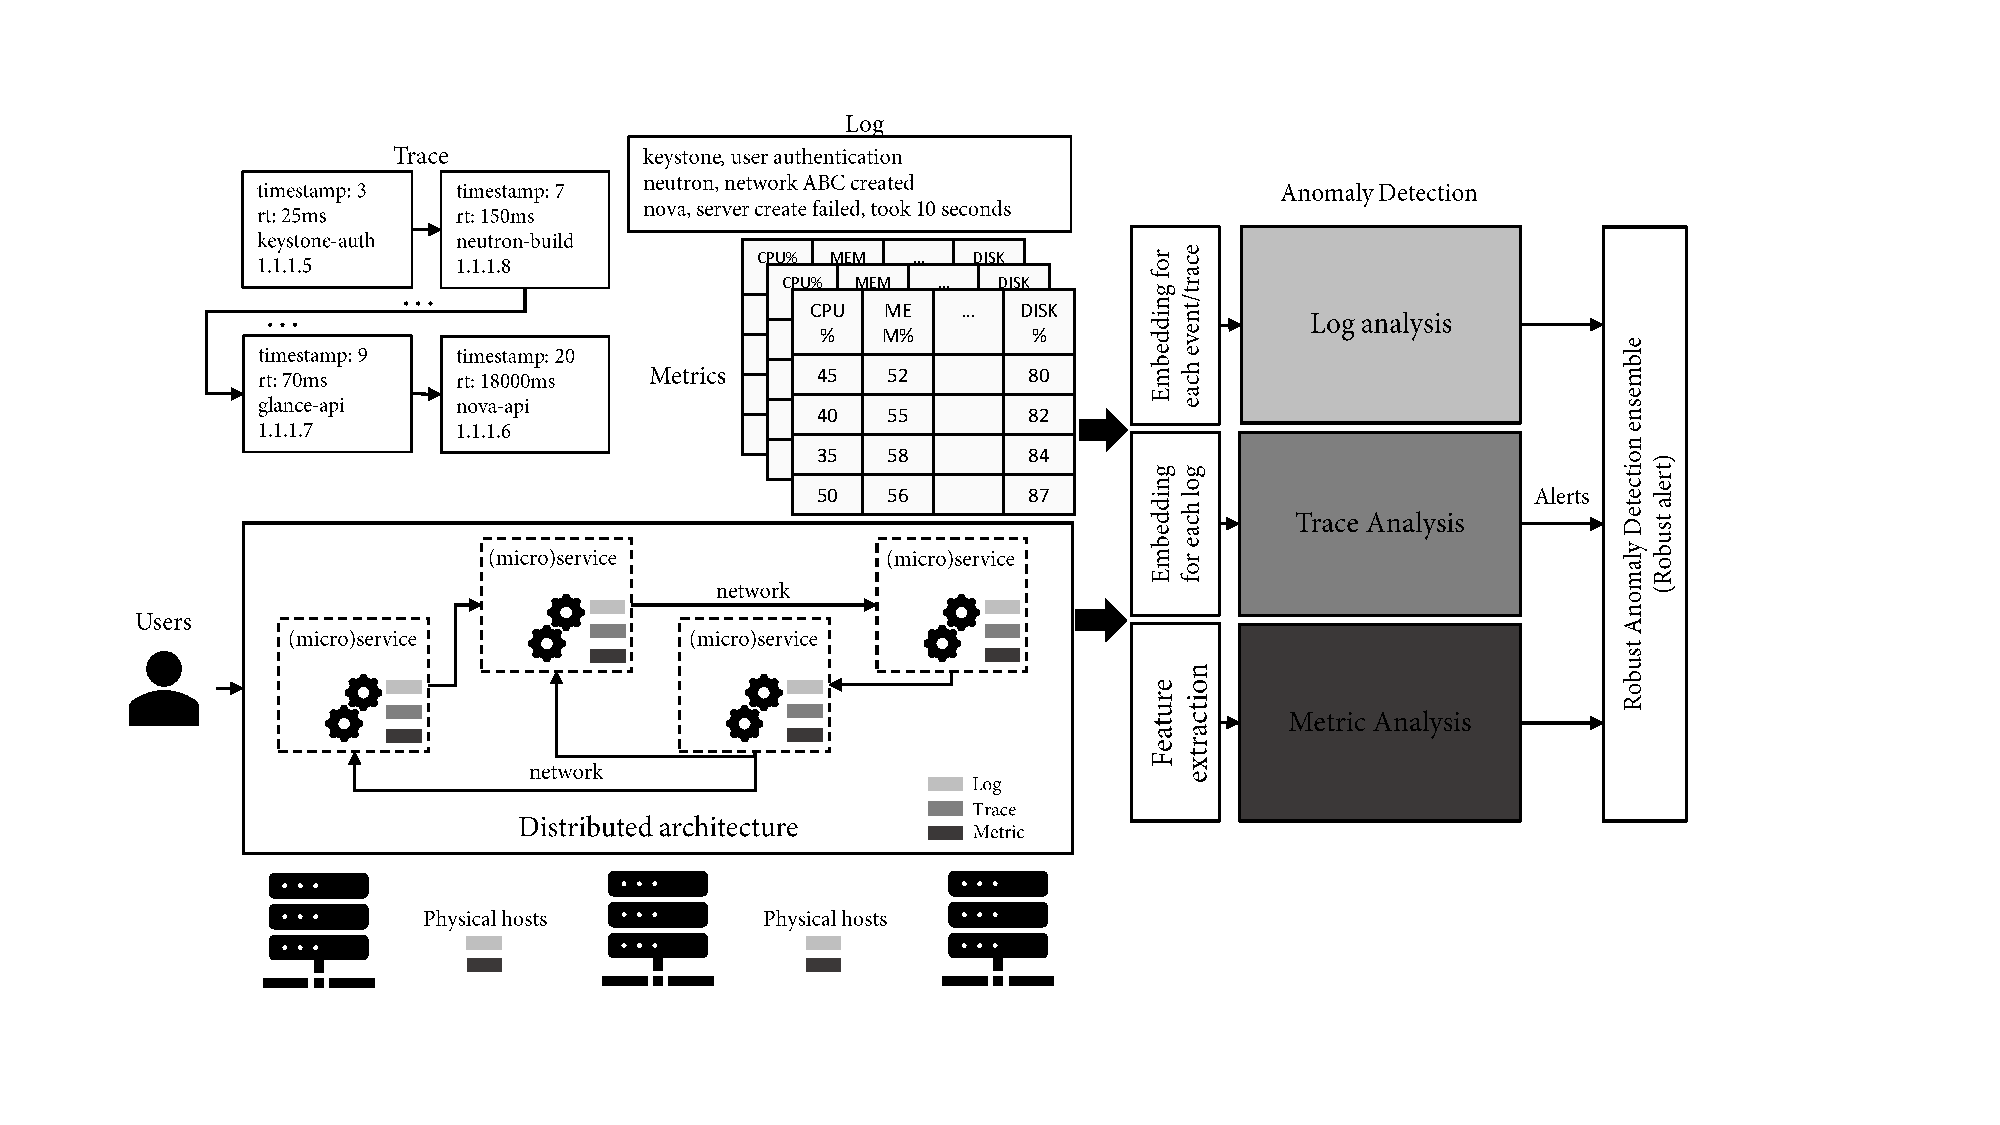
\includegraphics[width=1.0\textwidth]{gfx/chap2/solution_overview.pdf}}
\caption{Overview of the approach.}
\label{fig:solution_overview}
\end{figure}

\begin{enumerate}
    \item Log analysis:  Recent studies have focused predominantly on one-class deep learning methods on predefined non-learnable numerical log representations. The main limitation is that these models are not able to learn log representations describing the semantic differences between normal and anomaly logs, leading to a poor generalization of unseen logs. First, we propose NuLog~\cite{nedelkoski2020selfsupervised}, a log parser, which at the time of the writing of the thesis is state of the art in parsing task. NuLog's architecture enables learning log representations. We re-use the core architecture of NuLog in the novel log anomaly detection method, Logsy, a classification-based method to learn log representations in a way to distinguish between normal data from the system of interest and anomaly samples from auxiliary log datasets, easily accessible via the internet. The idea behind such an approach to anomaly detection is that the auxiliary dataset is sufficiently informative to enhance the representation of the normal data, yet diverse to regularize against overfitting and improve generalization. We propose an attention-based encoder model with a new hyperspherical loss function. This enables learning compact log representations capturing the intrinsic differences between normal and anomaly logs. Empirically, we show improvement by a large margin compared to the previous methods.
    \item Trace analysis:
    The concept of Artificial Intelligence for IT Operations (AIOps) combines big data and machine learning methods to replace a broad range of IT operations including availability and performance monitoring of services. Such platforms typically use separate models for each modality of monitoring data (e.g., textual properties and real-valued response time in logs and traces) to detect faults and upcoming anomalies in cloud services, which do not capture the existing correlation between the modalities. This paper extends the range of utilized data types for creation of a single model to improve the anomaly detection. We use a bimodal distributed tracing data from large cloud infrastructures in order to detect an anomaly in the execution of system components. We propose an anomaly detection method, which utilizes a single modality of the data with information about the trace structure. In the next step, we extend the single-modality neural architecture to a multimodal neural network with long short-term memory (LSTM) to enable the learning from the sequential nature of both modalities in the tracing data. Furthermore, we demonstrate an approach to detect dependent and concurrent events using the ability of the model to reconstruct the execution path. The implemented prototype is experimentally evaluated with data from a large-scale production cloud. The results demonstrate that the novel approaches outperform other deep-learning methods based on traditional architectures.
    \item Metric analysis:
     This paper presents an application-agnostic system to locate the culprits for microservice performance degradation with fine granularity, including not only the anomalous service from which the performance issue originates but also the culprit metrics that correlate to the service abnormality. Our method first finds potential culprit services by constructing a service dependency graph and next applies an autoencoder to identify abnormal service metrics based on a ranked list of reconstruction errors. Our experimental evaluation based on injection of performance anomalies to a microservice benchmark deployed in the cloud shows that our system achieves a good diagnosis result, with 92\% precision in locating culprit service and 85.5\% precision in locating culprit metrics.
\end{enumerate}

The proposed framework, as described, provides accurate anomaly detection, improved over the previous state-of-the-art, in the separate methods. However, to further improve the performance, and reduce the number of false predictions, we take a step further and propose an integrated solution via ensemble of these predictors. The ensemble enables more robust alerting compared to the single predictors. Given that all three sources originate from the same distributed system and are complementary, we propose a strategy to integrate them in one single prediction.

